\documentclass[a4paper,
               %boxit,
               %titlepage,   % separate title page
               %refpage      % separate references
              ]{jacow}
%
% CHANGE SEQUENCE OF GRAPHICS EXTENSION TO BE EMBEDDED
% ----------------------------------------------------
% test for XeTeX where the sequence is by default eps-> pdf, jpg, png, pdf, ...
%    and the JACoW template provides JACpic2v3.eps and JACpic2v3.jpg which
%    might generates errors, therefore PNG and JPG first
%
\makeatletter%
	\ifboolexpr{bool{xetex}}
	 {\renewcommand{\Gin@extensions}{.pdf,%
	                    .png,.jpg,.bmp,.pict,.tif,.psd,.mac,.sga,.tga,.gif,%
	                    .eps,.ps,%
	                    }}{}
\makeatother

% CHECK FOR XeTeX/LuaTeX BEFORE DEFINING AN INPUT ENCODING
% --------------------------------------------------------
%   utf8  is default for XeTeX/LuaTeX 
%   utf8  in LaTeX only realises a small portion of codes
%
\ifboolexpr{bool{xetex} or bool{luatex}} % test for XeTeX/LuaTeX
 {}                                      % input encoding is utf8 by default
 {\usepackage[utf8]{inputenc}}           % switch to utf8

\usepackage[USenglish]{babel}			 

\usepackage[final]{pdfpages}
\usepackage{multirow}
\usepackage{ragged2e}

%
% if BibLaTeX is used
%
\ifboolexpr{bool{jacowbiblatex}}%
 {%
  \addbibresource{jacow-test.bib}
  \addbibresource{biblatex-examples.bib}
 }{}
\listfiles

%
% command for typesetting a \section like word
%
\newcommand\SEC[1]{\textbf{\uppercase{#1}}}

%%
%%   Lengths for the spaces in the title
%%   \setlength\titleblockstartskip{..}  %before title, default 3pt
%%   \setlength\titleblockmiddleskip{..} %between title + author, default 1em
%%   \setlength\titleblockendskip{..}    %afterauthor, default 1em

%\copyrightspace %default 1cm. arbitrary size with e.g. \copyrightspace[2cm]

% testing to fill the copyright space
%\usepackage{eso-pic}
%\AddToShipoutPictureFG*{\AtTextLowerLeft{\textcolor{red}{COPYRIGHTSPACE}}}

\begin{document}

\title{preparation OF papers for \NoCaseChange{JACoW} conferences\thanks{Work supported by ...}}

\author{A. N. Author\thanks{email address}, H. Co-author, Name of Institute or Affiliation, City, Country \\
		P. Contributor\textsuperscript{1}, Name of Institute or Affiliation, City, Country \\
		\textsuperscript{1}also at Name of Secondary Institute or Affiliation, City, Country}
	
\maketitle

%
\begin{abstract}
   Many conference series have adopted the same standards
   for electronic publication and have joined the Joint
   Accelerator Conferences Website (JACoW) collaboration
   for the publication of their proceedings. This document
   describes the common requirements for the submission of
   papers to these conferences. Please consult individual
   conference information for page limits, method of electronic
   submission, etc. It is not intended that this should
   be a tutorial in word processing; the aim is to explain the
   particular requirements for electronic publication at
   www.JACoW.org.
\end{abstract}


\section{SUBMISSION OF PAPERS}
Each author should submit the PDF file and all source
files (text and figures) to enable the paper to be
reconstructed if there are processing difficulties.

\section{Manuscripts}
Templates are provided for recommended software and
authors are advised to use them. Please consult the
individual conference help pages if questions arise.

\subsection{General Layout}

These instructions are a typical implementation of the
requirements. Manuscripts should have:
\begin{Itemize}
    \item  Either A4 (\SI{21.0}{cm}~$\times$~\SI{29.7}{cm}; \SI{8.27}{in}~$\times$~\SI{11.69}{in}) or US
           letter size (\SI{21.6}{cm}~$\times$~\SI{27.9}{cm}; \SI{8.5}{in}~$\times$~\SI{11.0}{in}) paper.
    \item  Single-spaced text in two columns of \SI{82.5}{mm} (\SI{3.25}{in}) with \SI{5.3}{mm}
           (\SI{0.2}{in}) separation. More recent versions of MSWord have a default spacing of 1.5 lines;
           authors must change this to 1 line.
    \item  The text located within the margins specified in Table~\ref{l2ea4-t1}.
\end{Itemize}
\begin{table}[hbt]
%   \vspace*{-.5\baselineskip}
   \centering
   \caption{Margin Specifications}
   \begin{tabular}{lcc}
       \toprule
       \textbf{Margin} & \textbf{A4 Paper}                      & \textbf{US Letter Paper} \\
       \midrule
           Top         & \SI{37}{mm} (\SI{1.46}{in})            & \SI{0.75}{in} (\SI{19}{mm})        \\ %[3pt]
          Bottom       & \SI{19}{mm} (\SI{0.75}{in})            & \SI{0.75}{in} (\SI{19}{mm})        \\ %[3pt]
           Left        & \SI{20}{mm} (\SI{0.79}{in})            & \SI{0.79}{in} (\SI{20}{mm})        \\ %[3pt]
           Right       & \SI{20}{mm} (\SI{0.79}{in})            & \SI{1.02}{in} (\SI{26}{mm})        \\
       \bottomrule
   \end{tabular}
   \label{l2ea4-t1}
%   \vspace*{-\baselineskip}
\end{table}

\subsection{Fonts}

In order to produce good Adobe Acrobat PDF files, authors
using the LaTeX template are asked to use only the fonts
defined in the class file in standard, bold (i.\,e. \verb|\textbf|)
or italic (i.\,e., \verb|\textit|) form and
symbols from the standard set of fonts. In Word use only
Symbol and, depending on your platform, Times or Times New Roman
fonts in standard, bold or italic form.

The layout of the text on the page is illustrated in
Fig.~\ref{l2ea4-f1}. Note that the paper’s title and the author list should
be the width of the full page. Tables and figures may span
the whole \SI{170}{mm} page width, if desired (see Fig.~\ref{l2ea4-f2}), but
if they span both columns, they should be placed at either
the top or bottom of a page to ensure proper flow of the
text (Word templates only: the text should flow from top
to bottom in each column).

\begin{figure}[!htb]
%   \vspace*{-.5\baselineskip}
   \centering
   \includegraphics*[width=174pt]{JACpic_mc}
   \caption{Layout of papers.}
   \label{l2ea4-f1}
%   \vspace*{-\baselineskip}
\end{figure}

\begin{figure*}[!tbh]
    \centering
    \includegraphics*[width=\textwidth]{JACpic2v5}

    \caption{Example of a full-width figure showing the JACoW Team at their annual
    	     meeting in 2015. This figure has a multi-line caption that has to be
    	     justified rather than centred.}
    \label{l2ea4-f2}
%    \vspace*{-\baselineskip}
\end{figure*}

\subsection{Title and Author List}

The title should use \SI{14}{pt} bold uppercase letters and be centred on the page.
Individual letters may be lowercase to avoid misinterpretation (e.\,g., mW, MW, SPRing-8, SwissFEL).
To include a funding support statement, put an asterisk after the title and
the support text at the bottom of the first column on page~1---in Word,
use a text box; in \LaTeX, use $\backslash$\texttt{thanks}. See also the
subsection on footnotes.

The names of authors, their organizations/affiliations and
postal addresses should be grouped by affiliation and
listed in \SI{12}{pt} upper- and lowercase letters. The name of
the submitting or primary author should be first, followed
by the co-authors, alphabetically by affiliation. Where
authors have multiple affiliations, the secondary affiliation
may be indicated with a superscript, as shown in the
author listing of this paper. See \SEC{Annex~A} for further examples.

\subsection{Section Headings}

Section headings should not be numbered. They should
use  \SI{12}{pt}  bold  uppercase  letters  and  be  centred  in  the
column. All section headings should appear directly above
the text---there should never be a column break between a heading and the
following paragraph.

\subsection{Subsection Headings}

Subsection  headings  should  not  be  numbered.
They should use \SI{12}{pt} italic letters and be left aligned in the column.
Subsection headings use Title Case (or Initial Caps)
and should appear directly above the text---there should never be a column break
between a heading and the following paragraph.

\subsubsection{Third-level Headings} These should use \SI{10}{pt} bold
letters and be run into the paragraph text. In \LaTeX{} they are
created with \LaTeX's \verb|\subsubsection|LaTeX’s command.
In the Word templates authors must bold the heading text themselves.
This heading should be used sparingly. See Table~\ref{style-tab}
for its style details.

\subsection{Paragraph Text}

Paragraphs should use \SI{10}{pt} font and be justified (touch each side) in
the column. The beginning of each paragraph should be indented
approximately \SI{0.33}{cm} (\SI{0.13}{in}). The last line of a paragraph should not be
printed by itself at the beginning of a column nor should the first line of
a paragraph be printed by itself at the end of a column.

\subsection{Figures, Tables and Equations}

Place figures and tables as close to their place of mention as
possible. Lettering in figures and tables should be large enough to
reproduce clearly. Use of non-approved fonts in figures can lead to
problems when the files are processed. \LaTeX\ users should be sure to use
non-bitmapped versions of Computer Modern fonts in equations (Type\,1 PostScript
or OpenType fonts are required, Their use is described in the JACoW help
pages~\cite{jacow-help}).

Each figure and table must be numbered in ascending
order (1, 2, 3, etc.) throughout the paper. After inserting a
figure in a Word document, click on the figure, right click
on “Wrap Text”, and select the “In Line with Text” option.
Figure captions are placed below figures, and table
captions are placed above tables.

Figure captions are formatted as shown in Figs.~\ref{l2ea4-f1} and \ref{l2ea4-f2},
while table captions take the form of a heading,
with initial letters of principle words, capitalised, and
without a period at the end (see Tables~\ref{eq:units} and \ref{style-tab}).
Any reference to the contents of the table should be made from
the body of the paper rather than from within the table
caption itself.

 Single-line captions are centered in the column, while captions
that span more than one line should be justified.
The \LaTeX\ template uses the ‘booktabs’ package to
format tables.

When referring to a figure from within the text, the
convention is to use the abbreviated form [e.\,g., Fig.~1]
unless the reference is at the start of the sentence, in
which case “Figure” is written in full. Reference to a
table, however, is never abbreviated [e.\,g., Table~1].


If a displayed equation needs a number (i.\,e., it will be
referenced), place it it in parentheses, and flush with the
right margin of the column. The equation itself should be
indented and centred, as far as is possible:
\begin{equation}\label{eq:units}
    C_B=\frac{q^3}{3\epsilon_{0} mc}=\SI{3.54}{\micro eV/T}
\end{equation}

When referencing a numbered equation, use the word
“Equation” at the start of a sentence, and the abbreviated
form, “Eq.”, if in the text. The equation number is placed
in parentheses [e.g., Eq. (1)].

\subsection{Units}
	
Units should be written using the standard, roman font,
not the italic font, as shown in Eq.~(\ref{eq:units}).
An unbreakable space should precede a unit (in \LaTeX\ use a “\verb|\,|”,
the template uses the ‘siunits’ package to format units).
Some examples are: \SI{3}{keV},
\SI{100}{kW}, \SI{7}{µm}. When a unit appears in a hyphenated,
compound adjective that precedes a noun, it takes on the
singular form, e.\,g., the 3.8-metre long undulator.

\subsection{References}
%
% References examples given here are not formatted using \cite as there
%			 are only reference numbers [1] and [2] in the template
%
All bibliographical and web references should be numbered and listed at the
end of the paper in a section called \SEC{References}. When citing a
reference in the text, place the corresponding reference number in square
brackets~[1]. The reference citations in the text should be numbered
in ascending order. Multiple citations should appear in
the same square bracket~[3, 4] and
with ranges where appropriate~[1--4, 10].

A URL may be included as part of a reference, but its
hyperlink should NOT be added. The usual practice is to
use a monospace font for the URL so as to help distinguish
it from normal text. The Word template uses the
Lucida Sans Typewriter font (size \SI{8}{pt}), while the ‘url’ 
package in \LaTeX\ uses the Latin Modern Typewriter font.

For authors to properly cite the resources used when researching
their papers is an obligation. In the interest of
promoting uniformity and complete citations, the IEEE
Editorial Style for Transactions and Journals has been
adopted~\cite{IEEE}. Please consult the appended material, \SEC{Annex~B},
for details. The onus is on authors to pay attention to
the details of the said style to ensure complete, accurate
and properly formatted references.

\subsection{Footnotes}

Footnotes on the title and author lines may be used for acknowledgements,
affiliations and e-mail addresses. A non-numeric sequence of characters (*, \#,
\dag, \ddag) should be used.
Word users---DO NOT use Word's footnote feature (\textbf{Insert}, \textbf{Footnote})
to insert footnotes, as this will create formatting problems. Instead, insert
the title or author footnotes manually in a text box at the bottom of the first column with a
line at the top of the text box to separate the footnotes from the rest of
the paper's text.  The easiest way to do this is to copy the text box from
the JACoW template and paste it into your own document.
These “pseudo footnotes” in the text box should only
appear at the bottom of the first column on the first page.

Any other footnote in the body of the paper should
use the normal numeric sequencing (i.\,e., 1, 2, 3)
and appear at the bottom of the same column in which
it is used.

\subsection{Acronyms}

Acronyms should be defined the first time they appear.

\section{styles}

Table~\ref{style-tab} summarises the fonts and spacings used in the styles of
a JACoW template. In \LaTeX, these are implemented in the ‘jacow’ class file).

\section{page numbers}

\textbf{DO NOT include any page numbers}. They will be added
when the final proceedings are produced.

\begin{table}[h!t]
	\setlength\tabcolsep{3.5pt}
	\centering
	\caption{Summary of Styles}
	\label{style-tab}
	%    \begin{tabular}{p{60pt}p{90pt}cc}
	\begin{tabular}{llcc}
		\toprule
		\textbf{Style} & \textbf{Font}               & \textbf{Space}  & \textbf{Space} \\
		&                             & \textbf{Before} & \textbf{After} \\
		\midrule
		\textbf{PAPER}  & \SI{14}{pt}                 & \SI{0}{pt}      & \SI{3}{pt}  \\
		\textbf{TITLE}  & \textbf{UPPERCASE}          &                 &      \\
		& \textbf{EXCEPT FOR}         &                 &      \\
		& \textbf{REQUIRED lowercase} &                 &      \\
		& \textbf{letters}            &                 &      \\
		& \textbf{Bold}               &                 &      \\[5pt]
		%\midrule
		Author list  & \SI{12}{pt}                 & \SI{9}{pt}      & \SI{12}{pt} \\
		& UPPER- and lowercase        &                 &      \\[5pt]
		%\midrule
		\textit{Abstract} & \SI{12}{pt}                 & \SI{0}{pt}      & \SI{3}{pt} \\
		\textit{Title}  & \textit{Initial Caps}       &                 &      \\
		& \textit{Italic}             &                 &      \\[5pt]
		%\midrule
		\textbf{Section}  & \SI{12}{pt}                 & \SI{9}{pt}      & \SI{3}{pt}  \\
		\textbf{Heading}  & \textbf{UPPERCASE}          &                 &      \\
		& \textbf{bold}               &                 &      \\[5pt]
		%\midrule
		\textit{Subsection} & \SI{12}{pt}                 & \SI{6}{pt}      & \SI{3}{pt}  \\
		\textit{Heading}  & \textit{Initial Caps}       &                 &      \\
		& \textit{Italic}             &                 &      \\[5pt]
		%\midrule
		\textbf{Third-level} & \SI{10}{pt}                 & \SI{6}{pt}      & \SI{0}{pt}  \\
		\textbf{Heading}     & \textbf{Initial Caps}       &                 &      \\
		& \textbf{Bold}               &                 &      \\[5pt]
		%\midrule
		Figure        & \SI{10}{pt}                 & \SI{3}{pt}      & $\ge$\SI{3}{pt}  \\
		Captions      &                             &                 &      \\[5pt]
		%\midrule
		Table         & \SI{10}{pt}                 & $\ge$\SI{3}{pt} & \SI{3}{pt}  \\
		Captions      &                             &                 &      \\[5pt]
		%\midrule
		Equations     & \SI{10}{pt} base font       & \SI{12}{pt}     & \SI{12}{pt} \\[5pt]
		%\midrule
		References\footnotemark    
		& \SI{9}{pt}, justified with  & \SI{0}{pt}      & \SI{0}{pt} \\
		& \SI{0.52}{cm} (\SI{0.2}{in}) hanging       &                 &  \\
		& indent                      &                 &        \\
		\bottomrule   %\SI{0.25}{in}
	\end{tabular}
\end{table}
\footnotetext{In the case of more than 9 references, to ensure their proper alignment,
	Refs. 1 to 9 only should also have a \SI{0.16}{cm} (\SI{0.06}{in}) left indent, while Refs. 10
	onwards should have their hanging indent increased to \SI{0.68}{cm} (\SI{0.26}{in}). Further
	information is given in \SEC{Annex~B}.}

\section{templates}

Template documents for the recommended word processing
software are available from the JACoW website~\cite{jacow-help}
and exist for \LaTeX, Microsoft Word (Mac and PC)
and LibreOffice/Apache OpenOffice for US letter and A4
paper sizes.

Use the correct template for your paper size and version
of Word. Do not transport Microsoft Word documents across
platforms (e.\,g., Mac\,$\leftrightarrow$\,PC). To ensure
that fonts are embedded in Word 2010 documents (PC), the
“Embed fonts in file” option must be selected from within the
Word Options$\rightarrow$Save window. Fonts are embedded by
default when printing to PDF on MAC OSX.


\section{checklist for electronic publication}

\begin{Itemize}
	\item  Use only Times or Times New Roman (standard, bold or italic) and Symbol
	fonts for text---\SI{10}{pt} minimum except references, which can be \SI{9}{pt} or \SI{10}{pt}.
	\item  Figures should use Times or Times New Roman (standard, bold or italic) and
	Symbol fonts when possible---\SI{6}{pt} minimum.
	\item  Check that citations to references appear in sequential order and
	that all references are cited.
	\item  Check that the PDF file prints correctly.
	\item  Check that there are no page numbers.
	\item  Check that the margins on the printed version are within \SI{\pm1}{mm}
	of the specifications.
	\item  \LaTeX\ users can check their margins by invoking the
	\texttt{boxit} option.
\end{Itemize}

\raggedend
\newpage

\section{Conclusion}

Any conclusions should be in a separate section directly preceding
the \SEC{Acknowledgement}, \SEC{Appendix}, or \SEC{References} sections, in that
order.

\section{acknowledgement}
Any acknowledgement should be in a separate section directly preceding
the \SEC{References} or \SEC{Appendix} section.


\section{appendix}
Any appendix should be in a separate section directly preceding
the \SEC{References} section. If there is no \SEC{References} section,
this should be the last section of the paper.

\iffalse  % only for "biblatex"
	\newpage
	\printbibliography

% "biblatex" is not used, go the "manual" way
\else

%\begin{thebibliography}{99}   % Use for  10-99  references
\begin{thebibliography}{9} % Use for 1-9 references

%\bibitem{accelconf-ref}
%	C. Petit-Jean-Genaz and J. Poole,
%	``JACoW, A service to the Accelerator Community,''
%	EPAC'04, Lucerne, July 2004, THZCH03,  p.~249,
%	\url{http://www.JACoW.org/e04/papers/THZCH03.PDF}

\bibitem{jacow-help}
	JACoW,
	\url{http://www.jacow.org}

\bibitem{IEEE}
	\textit{IEEE Editorial Style Manual},
	IEEE Periodicals, Piscataway,
	NJ, USA, Oct. 2014, pp. 34--52.
\end{thebibliography}
%\null  % this is a hack for correcting the wrong un-indent by package 'flushend' in versions before 2015

\fi

\newpage

\twocolumn[\vspace*{-1.8ex}\section{ANNEX A:\endgraf FORMATTING OF AUTHORS AND AFFILIATIONS}]

The names of authors, their organizations/affiliations
and postal addresses should be grouped by affiliation and
listed in \SI{12}{pt} upper- and lowercase letters. The name of
the submitting or primary author should be first, followed
by the co-authors, alphabetically by affiliation. If the
author list for a given affiliation spans multiple lines,
please be sure to break the line in a manner that does not
split the author’s initials from the author’s last name. This
is easily done by placing unbreakable spaces between the
initials and last name. The affiliation name and address
are also best kept together on the same (but not necessarily
separate) line, wherever possible. (See, for example,
the entry for GSI in the following). In cases where authors
have multiple affiliations, the secondary affiliation is
inserted below the author/primary affiliation listing and is
indicated with a superscript, as shown in the following. A
spacing of \SI{3}{pt} is added to before the secondary affiliation.

\newpage

Footnotes on the title and author lines may be used for
acknowledgements and e-mail addresses, using a nonnumeric
sequence of characters (\textsuperscript{*}, \textsuperscript{†}, 
\textsuperscript{‡}, \textsuperscript{§}, \textsuperscript{\#}). In Word,
footnotes are best inserted manually in a text box at the
bottom of the first column with a line at the top of the text
box to separate the footnotes from the rest of the paper’s
text.

For examples of the preferred formatting of authors and
affiliations, please consult the following list of JACoW
collaboration members.

For manuscripts submitted by large collaborations with
potentially many tens of authors and where, additionally,
there may be page number limitations, a format consisting
of the principle author’s name and institute, followed by
“on behalf of the … collaboration”, is preferred.


\clearpage
%
% Include the title/author page of the JACoW Coolaboration
%
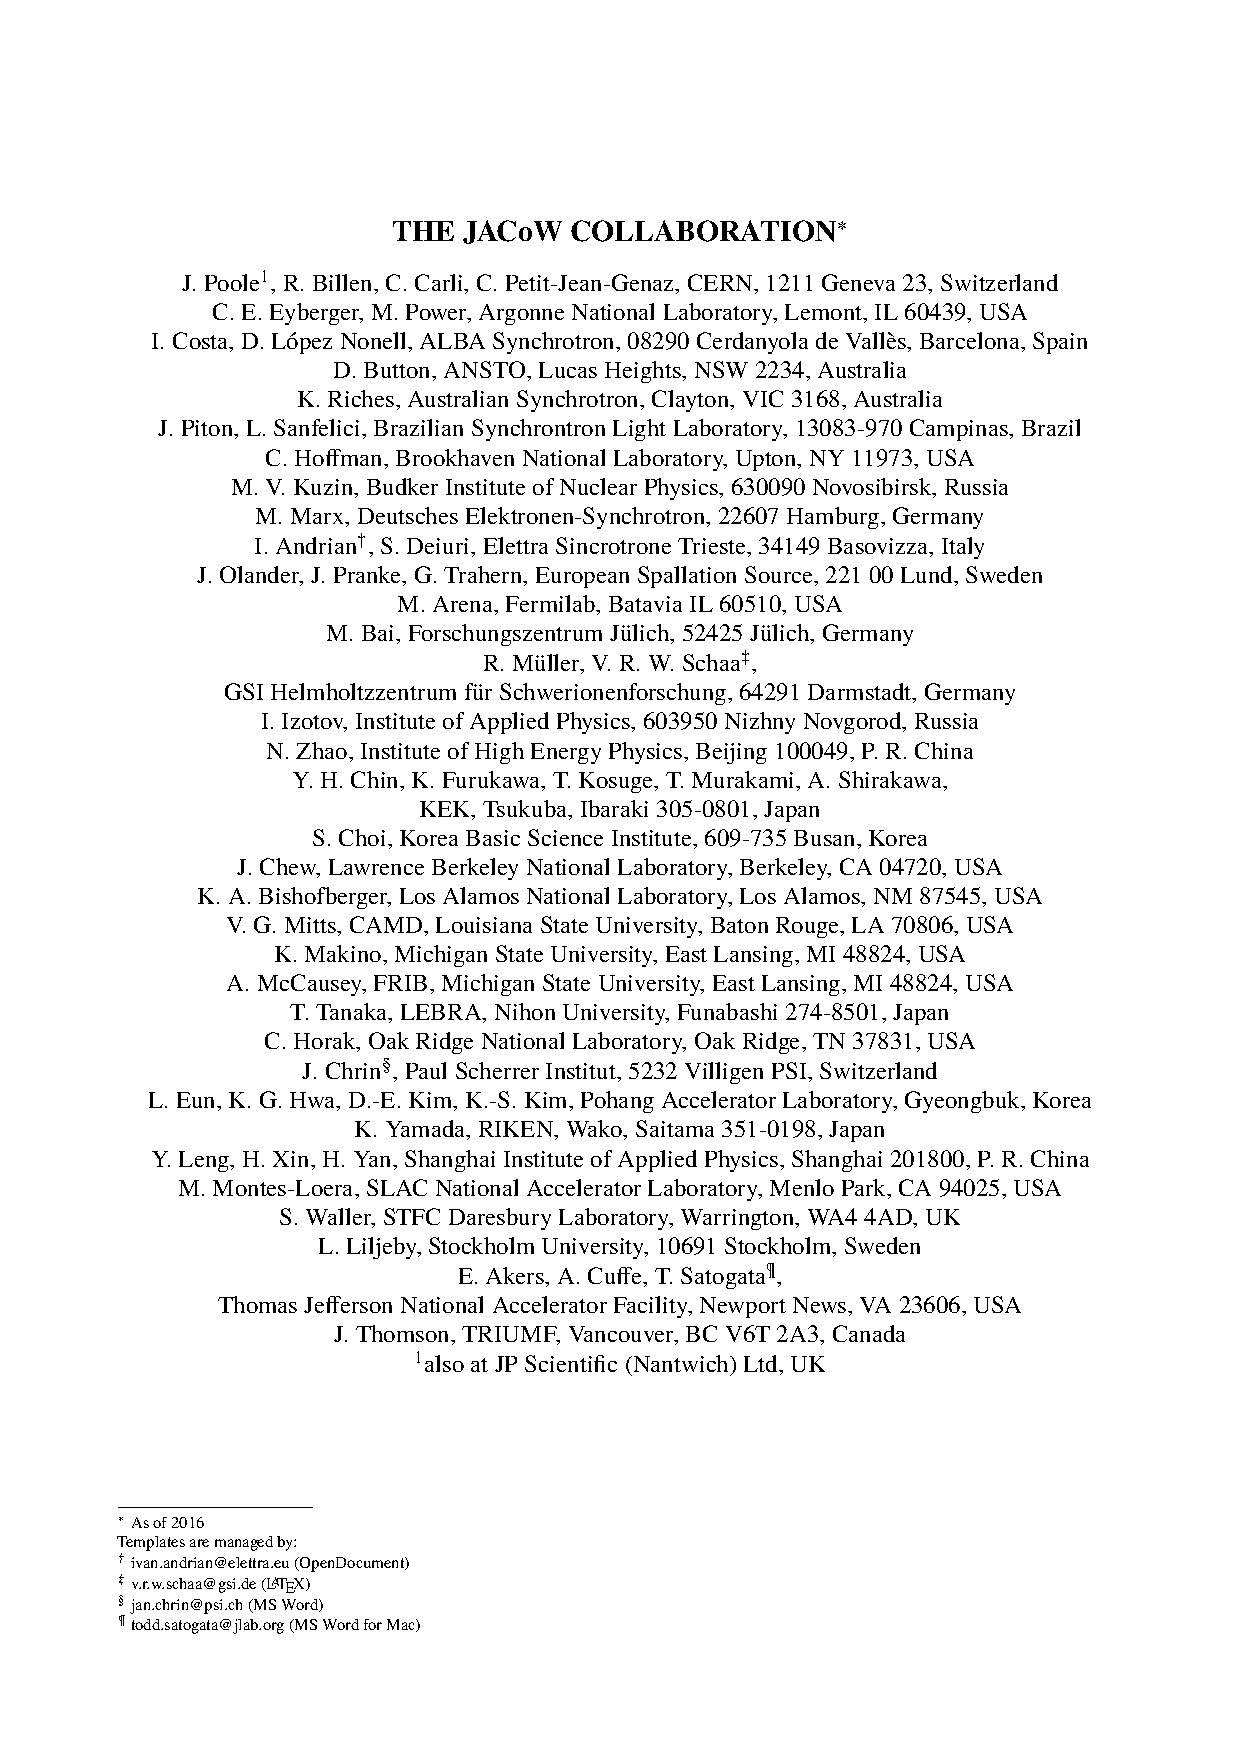
\includepdf[pages=-, noautoscale, pagecommand={}]{jacow-collaboration-2016.pdf}{}

\clearpage

\twocolumn[\vspace*{-1.8ex}\section{ANNEX B:\endgraf IEEE REFERENCE STYLE GUIDE AS APPLIED TO \NoCaseChange{JACoW} 
	PAPERS, PERIODICALS AND OTHER WORKS}]


\subsection{Referencing JACoW Proceedings}

The format for published JACoW proceedings papers
can be readily deduced from Refs. [1-3].

\subsubsection{Author Listing} Careful attention should be given to the
placing of commas and the use of ‘and’ in the author list.
In particular, for the case of six or more authors
(Ref. [3]), a comma also follows the penultimate author.
The preference for ‘\emph{et al.}’\ takes precedence when the number
of authors becomes large (e.g., $>$6).

\subsubsection{Paper Title} As is modern practice in references, the title
of the paper is written in sentence case, i.e., only the
initial letter of the first word in the title is capitalised.
Proper nouns, however, also have a capital. Capital letters
appearing in acronyms likewise remain unaltered

\subsubsection{Conference Proceedings} The proceedings title is written
in title case in italics using standard abbreviations,
such as Int. and Conf. The preposition, “in”, in normal
font, precedes the proceedings title. The location,
i.e., city, state (if USA), and country of the conference
venue, the month (three-letter abbreviation) and the year
the conference took place, is then listed. Finally, details
pertaining to the paper itself, such as the conference paper
ID and mandatory page numbers are given. The conference
paper ID is optional, and may be included in the
interest of facilitating a search through internet search
engines. The complete or abbreviated form for citations,
as shown in the following section, is recommended. The
former is more informative to readers outside the immediate
conference sphere. Both forms, however, ensure a
proper import into digital libraries and information
sources such as INSPIRE, Scopus, and Google Scholar.
To this end, the minimal form is also listed for convenience.
Although this form is not advocated, it nevertheless
remains acceptable.

Authors are also reminded to make a distinction between
papers published in JACoW proceedings (which
will always have page numbers) and those papers that
may have been presented at past JACoW conferences but
were not published [4]. References to contributions presented
at the same conference should be written as shown
in Ref. [5]; the wording “this conference” may be optionally
appended.

\subsection{Referencing Periodicals and Other Sources}

The IEEE style is also shown for periodicals [6-11],
online sources [12], books [13, 14], internal reports [15],
theses [16], manuals or handbooks [17], patents [18] and
unpublished material [19, 20]. Examples of correctly
formatted references can be found at the JACoW website,
under ‘Formatting Citations’ which is reached through the
‘for Authors’ link.

\subsection{Alignment of References}

Entries to the References section follow a hanging indent
structure. In this way, reference numbers in the first
line of each reference entry are right aligned, while subsequent
lines within a given reference are indented by a
specified amount. The indentation values for Word are
shown in Table~1 of this Annex and depend on whether
the number of references exceeds single digit values.

In the \LaTeX\ template, \verb|\bibliography{9}| is used for
when the total number of references is less than ten. This
should be changed to \verb|\bibliography{99}| if the number of
references is ten or more.

\begin{table}[h!t]
	\centering
	%\setlength\tabcolsep{3.5pt}
	\caption{Formatting of References}
	\label{format-refs}
	%    \begin{tabular}{p{60pt}p{90pt}cc}
	\begin{tabular}{lllcc}
		\toprule
		\textbf{Font} & \textbf{Left}   & \textbf{Hanging}  & \textbf{Space}   & \textbf{Space} \\
		              & \textbf{Indent} & \textbf{Indent}   & \textbf{Before}  & \textbf{After} \\
		\midrule
		\multicolumn{5}{c}{\textbf{No. References $\le$9}}  \\
		\SI{9}{pt},   & \SI{0.00}{cm}   & \SI{0.52}{cm}     & \multirow{2}{*}{\SI{0}{pt}} 
																			   & \multirow{2}{*}{\SI{3}{pt}}  \\
		justified     & \SI{0.00}{in}   & \SI{0.20}{in}     &                  &             \\
		\midrule
		\multicolumn{5}{c}{\textbf{No. References $\ge$10}}  \\[1mm]
		\multicolumn{5}{l}{\textbf{Refs. 1 to 9}}           \\[1mm]
		\SI{9}{pt},   & \SI{0.16}{cm}   & \SI{0.52}{cm}     &  \multirow{2}{*}{\SI{0}{pt}} 
																			   & \multirow{2}{*}{\SI{3}{pt}}  \\
		justified     & \SI{0.06}{in}   & \SI{0.20}{in}     &                  &             \\[3mm]		\multicolumn{5}{l}{\textbf{Refs. 10 onwards}}    \\[1mm]
		\SI{9}{pt},   & \SI{0.00}{cm}   & \SI{0.68}{cm}     &  \multirow{2}{*}{\SI{0}{pt}} 
																	           & \multirow{2}{*}{\SI{3}{pt}}  \\
		justified     & \SI{0.00}{in}   & \SI{0.26}{in}     &                  &             \\
		\bottomrule  
	\end{tabular}
\end{table}

\patchcmd\thebibliography{\section*{REFERENCES\@mkboth {REFERENCES}{REFERENCES}}}{}{}{}
\section{PAPER PUBLISHED IN A CONFERENCE PROCEEDINGS}

\definecolor{jgreen}{cmyk}{0.81, 0.00, 0.97, 0.00}
\definecolor{jred}{cmyk}  {0.00, 0.99, 1.00, 0.00}
\definecolor{jgrepc}{cmyk}{0.74, 0.05, 1.00, 0.00}
\definecolor{jblue}{cmyk} {0.87, 0.54, 0.00, 0.00}
\definecolor{jvio}{cmyk}  {0.41, 0.82, 0.00, 0.00}
\definecolor{jbook}{cmyk} {0.28, 0.88, 0.79, 0.25}
\definecolor{jrept}{cmyk} {0.07, 0.70, 1.00, 0.00}
\definecolor{jmanu}{cmyk} {0.28, 0.77, 1.00, 0.23}
\definecolor{junpu}{cmyk} {0.00, 0.83, 0.65, 0.00}


\subsection{Complete Form}

%\begin{thebibliography}{99}   % Use for  10-99  references
\begin{thebibliography}{9} % Use for 1-9 references
	
	\bibitem{item:1-1}
	A.~Alpha and B.~T.~Beta, “An interesting paper”, 
	in \textit{Proc. 1st Int. Particle Accelerator Conf. (IPAC’10)}, 
	Kyoto, Japan, May 2010, 
	paper MOP057, pp. 567--569.\\
	\textcolor{jgreen}{[Conference Proceedings, two authors; optional paper ID]}

	\bibitem{item:1-2}
	A.~Alpha \emph{et al.}, 
	“A fascinating paper about FELs”, 
	in \emph{Proc. 35th Int. Free-Electron Laser Conf. (FEL’13)}, 
	New York, NY, USA, Aug. 2013, 
	paper WEP033, pp. 27--29.\\
	\textcolor{jgreen}{[Conference Proceedings, for six or more authors use \emph{et al.};	
		paper ID is optional]}
	
	\bibitem{item:1-3}	
	A.~Alpha, B.~T.~Beta, C.~Gamma, and D.~Delta, 
	“An overview of control systems”, 
	in \emph{Proc. 13th Int. Conf. on Accelerator and Large Experimental Physics Control Systems (ICALEPCS’11)}, Grenoble, France, Oct. 2011, 
	paper TUP014, pp. 89--91.\\
	\textcolor{jgreen}{[Conference Proceedings, four authors; optional paper ID]}
\end{thebibliography}

\newpage
\subsection{Abbreviated Form}

\begin{thebibliography}{9} % Use for 1-9 references
	\bibitem{item:2-1}
	A.~Alpha and B.~T.~Beta, “An interesting paper”, 
	in \textit{Proc. IPAC’10}, 
	Kyoto, Japan, May 2010, 
	paper MOP057, pp. 567--569.\\
	\textcolor{jgreen}{[Conference Proceedings, two authors; optional paper ID]}
	
	\bibitem{item:2-2}
	A.~Alpha \emph{et al.}, 
	“A fascinating paper about FELs”, 
	in \emph{Proc. FEL’13}, 
	New York, NY, USA, Aug. 2013, 
	paper WEP033, pp. 27--29.\\
	\textcolor{jgreen}{[Conference Proceedings, for six or more authors use \emph{et al.};	
		paper ID is optional]}
	
	\bibitem{item:2-3}	
	A.~Alpha, B.~T.~Beta, C.~Gamma, and D.~Delta, 
	“An overview of control systems”, 
	in \emph{Proc. ICALEPCS’11}, Grenoble, France, Oct. 2011, 
	paper TUP014, pp. 89--91.\\
	\textcolor{jgreen}{[Conference Proceedings, four authors; optional paper ID]}
\end{thebibliography}

\subsection{Minimal Form}

\begin{thebibliography}{9} % Use for 1-9 references

	\bibitem{item:3-1}
	A.~Alpha and B.~T.~Beta,
	in \textit{Proc. IPAC’10}, 
	pp. 567--569.\\
	\textcolor{jgreen}{[Conference Proceedings, two authors]}
	
	\bibitem{item:3-2}
	A.~Alpha \emph{et al.}, 
	in \emph{Proc. FEL’13}, 
	pp. 27--29.\\
	\textcolor{jgreen}{[Conference Proceedings, for six or more authors use \emph{et al.}]}
	
	\bibitem{item:3-3}	
	A.~Alpha, B.~T.~Beta, C.~Gamma, and D.~Delta, 
	in \emph{Proc. ICALEPCS’11}, 
	pp. 89--91.\\
	\textcolor{jgreen}{[Conference Proceedings, four authors]}
\end{thebibliography}

\section{UNPUBLISHED PAPER PRESENTED AT A PREVIOUS CONFERENCE}

\subsection{Complete Form}

\begin{thebibliography}{9} % Use for 1-9 references
\setcounter{enumi}{3}
 \bibitem{item:41}
	A.~Alpha and B.~T.~Beta, 
	“An interesting talk”, 
	presented at the 5th Int. Particle Accelerator Conf. (IPAC’14), 
	Dresden, Germany, Jun. 2014, paper MOP057, unpublished.\\
	\textcolor{jred}{[Unpublished paper; conference name in normal font; paper
	ID may only be given if material supplementing the proceedings
	exists on the JACoW website, e.\,g., PDF of talk]}
\end{thebibliography}

\subsection{Abbreviated Form}

\begin{thebibliography}{9} % Use for 1-9 references
\setcounter{enumi}{3}
 \bibitem{item:42}
	A.~Alpha and B.~T.~Beta, 
	“An interesting talk”, 
	presented at IPAC’14, 
	Dresden, Germany, Jun. 2014, paper MOP057, unpublished.\\
	\textcolor{jred}{[Unpublished paper; conference name in normal font; paper
	ID may only be given if material supplementing the proceedings
	exists on the JACoW website, e.\,g., PDF of talk]}
\end{thebibliography}


\section{PAPER PRESENTED AT THE CURRENT CONFERENCE}

\subsection{Complete Form}

\begin{thebibliography}{9} % Use for 1-9 references
\setcounter{enumi}{4}
 \bibitem{item:51}
	A.~Alpha and B.~T.~Beta, 
	“An interesting talk”, 
	presented at the 7th Int. Particle Accelerator Conf. (IPAC’16), 
	Busan, Korea, May 2016, 
	paper MOAB01, this conference.\\
	\textcolor{jgrepc}{[Current conference; conference name in normal font; the
			           wording “this conference” is optional]}
\end{thebibliography}

\subsection{Abbreviated Form}

\begin{thebibliography}{9} % Use for 1-9 references
\setcounter{enumi}{4}
	\bibitem{item:52}
	A.~Alpha and B.~T.~Beta, 
	“An interesting talk”, 
	presented at IPAC’16, 
	Busan, Korea, May 2016, 
	paper MOAB01, this conference.\\
	\textcolor{jgrepc}{[Current conference; conference name in normal font; the
		wording “this conference” is optional]}
\end{thebibliography}


\section{PAPER PUBLISHED IN, OR SUBMITTED TO, A PERIODICAL}

\begin{thebibliography}{99} % Use for 1-9 references
  \setcounter{enumi}{5}
	\bibitem{item:6}
		P.~Mercury \emph{et al.}, 
		“Title of paper published in journal”,
		\emph{Phy. Rev. Lett.}, vol. 114, no. 5, 
		p. 050511, Feb. 2014. \\
	\textcolor{jblue}{[Periodical, Phys. Rev. Lett.; 
		             issue no. and month may be omitted]}

	\bibitem{item:7}
		P.~Venus \emph{et al.}, 
		“New techniques in laser wakefield accelerators”,
		\emph{Phys. Rev. ST Accel. Beams}, vol. 18, 
		p. 120198, Dec.~2015.   \\
	\textcolor{jblue}{[Periodical, Phys. Rev. ST Accel. Beams; 
			              month may be omitted]}

	\bibitem{item:8}
		T.~Earth \emph{et al.}, 
		“Low dose irradiation impact on modern silicon detectors”, 
		\emph{Nucl. Instr. Meth.}, vol. 692, pp. 256--280, 2014.
	\textcolor{jblue}{[Periodical, Nucl. Instr. Method.]}
	
	\bibitem{item:9}
		T.~Earth, L.~Moon, and A.~Belt, 
		“Temporal correlations of x-ray free electron lasers”, 
		\emph{Optics Express}, vol. 20, pp. 11396--11404, 2012.
	\textcolor{jblue}{[Periodical, Optics Express]}

	\bibitem{item:10}
		J.~B.~Good, 
		“A paper accepted for publication”, 
		\emph{Phys. Rev. Lett.}, to be published.
	\textcolor{jblue}{[Periodical, paper accepted for publication 
		              by Phys. Rev. Lett.]}

	\bibitem{item:11}
		G.~D.~Read, 
		“Title of paper submitted for publication”,
		submitted for publication.
	\textcolor{jblue}{[Paper submitted for publication; the name of the 
					  periodical does not appear]}
\end{thebibliography}

\section{ONLINE SOURCE}

\begin{thebibliography}{99} % Use for 1-9 references
  \setcounter{enumi}{11}
	\bibitem{item:121}
		JACoW, \url{http://www.jacow.org} \\
		\textcolor{jvio}{[online source; no hyperlink, no period at end of URL
						  unless there is a trailing “/” as shown below. A monospace
						  font, such as Lucida Sans Typewriter (size 8 pt), is used in
					      Word, while the ‘url’ package in \LaTeX\ uses the Latin Modern Typewriter font]}

  \setcounter{enumi}{11}
	\bibitem{item:122}
		JACoW, \url{http://www.jacow.org/}.  \\
	\textcolor{jvio}{[online source; no hyperlink, period after traling “/” in
					 URL allowed. A monospace font, such as Lucida Sans Typewriter 
					 (size 8 pt), is used in Word, while the ‘url’ package in \LaTeX\  
					 uses the Latin Modern Typewriter font]}
\end{thebibliography}

\section{CITATIONS TO BOOKS}

\begin{thebibliography}{99} % Use for 1-9 references
	\setcounter{enumi}{12}
	\bibitem{item:13}
		T.~Earth and L.~Moon, 
		“Title of chapter in the book”, 
		in \emph{Title of Book}, R Mars, Ed. New York, NY, USA: 
		Wiley, 1994, pp.~42--48. \\
	\textcolor{jbook}{[Chapter in book]}
	
	\bibitem{item:14}
		A.~Belt, \emph{Title of Book}. Cambridge, MA, USA: 
		MIT Press, 1986. \\
	\textcolor{jbook}{[Book]}
\end{thebibliography}

\section{REPORTS AND THESES}

\begin{thebibliography}{99} % Use for 1-9 references
	\setcounter{enumi}{14}
	\bibitem{item:15}
		G. Jupiter \emph{et al.}, 
		“Title of report”, CERN, Geneva, Switzerland,
		Rep. CERN-2012-333, Oct. 2012.\\
	\textcolor{jrept}{[Report]}

	\bibitem{item:16}
		A.~Student, “Title of thesis”, 
		Ph.D. thesis, Phys. Dept.,
		Karlsruher Institut für Technologie, Karlsruhe, 
		Germany, 2014.\\
	\textcolor{jrept}{[Thesis]}
\end{thebibliography}

\newpage

\section{MANUAL}

\begin{thebibliography}{99} % Use for 1-9 references
	\setcounter{enumi}{16}
	\bibitem{item:17}
		\emph{IEEE Editorial Style Manual}, 
		IEEE Periodicals, 
		Piscataway, NJ, USA, Oct. 2014, pp. 34-52; 
		\url{http://www.ieee.org/documents/style_manual.pdf} \\
	\textcolor{jmanu}{[Handbook/Manual, no hyperlink, no period after URL]}
\end{thebibliography}

\section{PATENTS}

\begin{thebibliography}{99} % Use for 1-9 references
	\setcounter{enumi}{17}
		\bibitem{item:18}
		A.~N.~Inventor, 
		“Title of patent”, 
		Patent Authority and No., Jan. 20, 2016.

\end{thebibliography}

\newpage

\section{UNPUBLISHED WORK AND PRIVATE COMMUNICATION}

\begin{thebibliography}{99} % Use for 1-9 references
	\setcounter{enumi}{18}
	\bibitem{item:19}
		P.~Neptune, “Title of paper”, unpublished.\\
	\textcolor{junpu}{[Unpublished]}
	
	\bibitem{item:20}
	P.~Uranus, private communication, Jun. 2015.\\
	\textcolor{junpu}{[Private communication]}

\end{thebibliography}
\null  % this is a hack for correcting the wrong un-indent by package 'flushend' in versions before 2015

\newpage

\twocolumn[\vspace*{-1.8ex}\section{ANNEX C:\endgraf THE DILIGENT AUTHOR’S CHECKLIST}]

\subsection{Common Oversights}

In order to lessen the load on a small team of editors
and to help expedite publication of the Proceedings, authors
are kindly asked to give themselves an extra few
minutes to go over the following points, which highlight
the most common errors, before uploading their paper. By
providing a properly formatted JACoW paper, the Proceedings
Office is able to benefit from an autodistill process
which automatically converts the author's PDF file
into a version that adheres to the JACoW-compliant PDF
standard. The process further ensures that all fonts required
to view the entire document are embedded, rendering
a final PDF that qualifies technically for publication.


\subsection{Author and Affiliation Listing}

The names of authors and their affiliations should be in
\SI{12}{pt} uppercase and lowercase letters, with standard,
roman fonts (i.\,e., not italics). When there is more than
one author, the submitting author should be first, followed
by the co-author. Co-authors should be grouped by affiliation
and then be listed alphabetically. Please refer to \SEC{Annex~A}
for further details and examples, particularly for
the case where authors have multiple institutes.

\subsection{Title, Abstract, and Author Listing in the SPMS}

Authors are prompted to verify that the title, the abstract
and the author/institute listing, previously submitted
to the SPMS, has been updated to match that now appearing
in the final manuscript. In particular, primary authors
are reminded that it is their responsibility to check the
accuracy of the co-authors entered in the SPMS database.
These should be an exact match to that appearing in the
paper. This is required to ensure the proper indexing of
authors to papers in the published proceedings.

\subsection{Subsection Headings}

Subsection Headings use \SI{12}{pt} italic lowercase and uppercase.
The initial letter of every principle word is capitalised,
and the heading is left aligned in the column.

\subsection{Figure Captions}

Figure captions should be placed below the figure and
centered if on one line, but justified if spanning two or
more lines:
\begin{center}
	Figure 1: A one line figure caption is centered.
\end{center}
\begin{justify}
	Figure 2: A lengthy figure caption that spans 
	two lines is justified.
\end{justify}
Note the colon “:” after the figure number and the period
“.” at the end of the caption.

\newpage

When referring to a figure from within the text, the
convention is to use the abbreviated form, i.\,e., Fig.~1,
unless the reference to the figure is at the start of the sentence:
\begin{quote}
	Figure 1 shows a schematic view of...
	
	... as shown in Fig.~1.
\end{quote}

\subsection{Table Headings}

Table captions should be placed above the table and
centered if on one line, but justified if spanning two or
more lines:
\begin{center}
	Table 1: Table Heading
\end{center}
\begin{justify}
	Table 2: A Particularly Long Table Heading 
	Spanning Two Lines
\end{justify}

Note the colon ":" after the table number, that the initial
letters of the principle words in the table heading are
capitalised, and the absence of a period at the end of the
caption.

When referring to a table from within the text, the convention
is NOT to abbreviate, i.\,e., Table 1.

\subsection{Equations}

If a displayed equation requires a number, it should be
placed flush with the right margin of the column. Please
leave sufficient space immediately before and after the
equation, i.\,e., in Microsoft Word, \SI{12}{pt} before and after.

\subsection{Units}

An unbreakable space should always precede a unit. In \LaTeX\ use 
a “\verb|\,|” or the ‘siunits’ package to format units.
Examples are:
\SI{3}{keV}, \SI{4}{GeV}, \SI{100}{kW}, \SI{7}{µm}.

\subsection{References}

References are written in \SI{9}{pt} size and should be neatly
presented in a consistent format with reference numbers
aligned. Please refer to \SEC{Annex~B} for the preferred format
and proper alignment.

Please also ensure that references in the text are cited in
sequential order.


\end{document}
	